\section{System - PHP Framework}
\frame{
	\begin{block}{}
  	\begin{center}
  	\huge{System - PHP Framework}
	\end{center}
  	\end{block}
}			

\subsection{Anwendungsbereich}
\frame{
	\frametitle{Anwendungsbereich von System}
	System kann in PHP-basierten Anwendungen eingesetzt werden.
	\begin{block}{}
	\begin{itemize}
	\item{Websites}
   	\item{Webtools}
	\item{Webapps}
	\end{itemize}
	\end{block}
}

\subsection{Features}
\frame{
	\frametitle{Features von System}
	System vereichfacht die Entwicklung von PHP basierten Anwendungen
	\begin{block}{}
	\begin{itemize}
	\item{Kapselung}
   	\item{REST Schnittstelle}
	\item{Moderne Webtechnologien}
	\item{Utilities}
	\item{Modulare GUI für administrative Aufgaben}
	\end{itemize}
	\end{block}
	Teilintegration möglich
}
	
\subsubsection*{Kapselung}
\frame[t]{
	\frametitle{Klassische Struktur von PHP Projekten}
	Die klassische Struktur von PHP Projekten orientiert sich oft an der HTML Struktur.
	\begin{backgroundblock}{2.5cm}{4cm}
		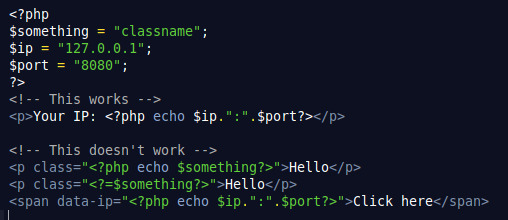
\includegraphics[width=8cm]{img/inlinehtml.jpg}
	\end{backgroundblock}
}
\frame{
	\frametitle{Klassische Struktur von PHP Projekten - Nachteile}
	\begin{block}{}
	\begin{itemize}
	\item{HTML Code ist unübersichtlich}
	\item{Programm ist eine Datei, zerteilt in Abschnitte}
	\item{Definitionen in anderen Abschnitten des Programms}
	\item{Spezialwissen notwendig für die Wartung}
	\end{itemize}
	\end{block}
}

\frame{
	\frametitle{Kapselung in System}
	Eine Gute Kapselung vereinfacht die Übersicht über das Programm.
	\begin{block}{}
		\begin{itemize}
			\item{nach Sprache}
			\item{nach Art der Rückgabe (Website/Daten/Administratives)}
			\item{Nach Sinneinheit (Seiten/Module)}
		\end{itemize}
	\end{block}
}

\frame[t]{
	\frametitle{Kapselung nach Sprache - MVC-Modell}
	\begin{quote}
		Der Begriff model view controller (MVC) ist ein Muster zur Strukturierung von Software-Entwicklung in die drei Einheiten Datenmodell, Präsentation und Programmsteuerung. (wikipedia)
	\end{quote}
	\begin{backgroundblock}{2.5cm}{5.0cm}
		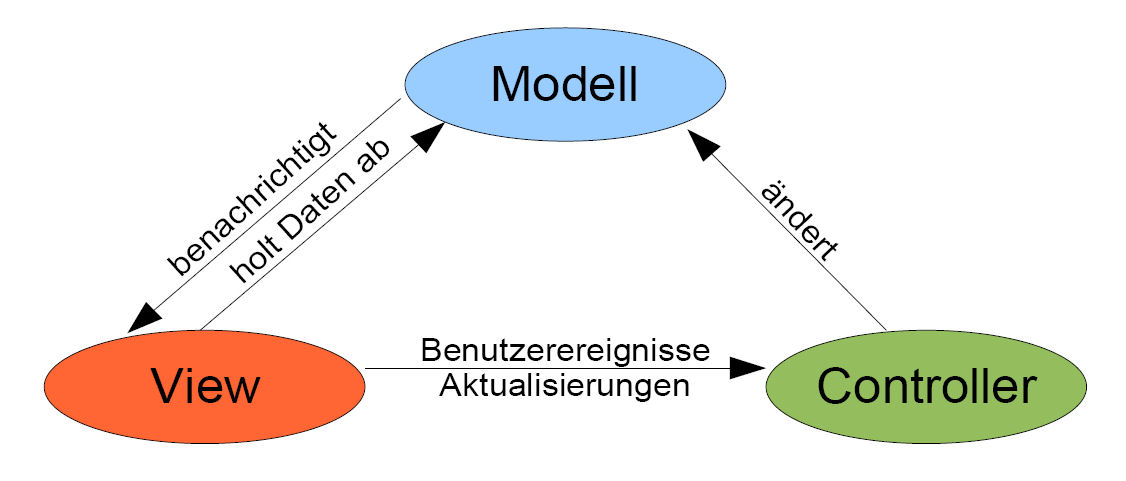
\includegraphics[width=7cm]{img/mvc.jpg}
	\end{backgroundblock}
}
	
\frame{
	\frametitle{Kapselung nach Sprache}
	Die Kapselung nach Sprache implementiert ein MVC-Modell
	\begin{block}{MVC durch Kapselung nach Sprache}
	\begin{itemize}							
		\item{PHP (Controller Server)}
		\item{SQL (Model)}
		\item{JS (Controller Client)}
		\item{CSS (View)}
		\item{HTML (View)}
	\end{itemize}
	\end{block}
}

\frame{
	\frametitle{Kapselung nach Art der Rückgabe}
	\begin{block}{Endpoints Kapseln die Rückgabe}
	\begin{itemize}
		\item{index.php - Webpages/HTML Rückgabe}
		\item{api.php - JSON-Daten/Steueranweisungen}
		\item{sai.php - Administrative Aufgaben}
		\item{(setup.php - Install Scripts)}
	\end{itemize}
	\end{block}
}

\frame[t]{
	\frametitle{Kapselung nach Sinneinheit}
	\begin{block}{}
	\begin{itemize}
		\item{Ordnerstrukturen ordnen den Code}
		\item{Modulare Schnittstellen - pages, sai module}
		\item{Frei wählbar}
	\end{itemize}
	\end{block}
	Das PHP-Feature ``autoload'' ermöglicht es \\
	Klassen bei Bedarf nachzuladen.
	\begin{backgroundblock}{9.0cm}{2.0cm}
		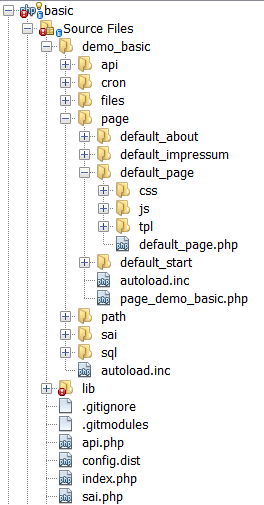
\includegraphics[width=3cm]{img/ordnerstruc.png}
	\end{backgroundblock}
}
	
\subsubsection*{REST in System}
\frame{
	\frametitle{REST in System - quality APIs}
	\begin{block}{Funktion}
	\begin{itemize}
	\item{Mapping von URL-Parametern auf Funktionsnamen}
	\item{Regeln definiert zulässige Aufrufe}
	\item{Parameter-Typ-Prüfung}
	\end{itemize}
	\end{block}
	
	\begin{block}{Nutzen}
	\begin{itemize}
	\item{Sicherheit}
	\item{Zuverlässigkeit}
	\item{Persistenz}
	\end{itemize}
	\end{block}
}

\subsubsection*{Moderne Webtechnologien in System}
\frame[t]{
	\frametitle{Moderne Webtechnologien, von System unterstützt}
	\begin{block}{}
	\begin{itemize}
	\item{Hashbang Crawling-Scheme - \#!adresse}
	\item{JQuery \& Bootstrap}
	\item{SCSS(SASS)}
	\item{Minify}
	\item{Git}
	\end{itemize}
	\end{block}
	%\begin{backgroundblock}{1.0cm}{6.5cm}
	%	
\includegraphics[width=1.5cm]{img/hashbangs.png}
	%\end{backgroundblock}
	\begin{backgroundblock}{1.0cm}{6.5cm}
		
\includegraphics[width=1.5cm]{img/jQurery.jpg}
	\end{backgroundblock}
	\begin{backgroundblock}{3.0cm}{6.8cm}
		
\includegraphics[width=1.5cm]{img/bootstrap-logo.png}
	\end{backgroundblock}
	\begin{backgroundblock}{5.0cm}{6.5cm}
		
\includegraphics[width=1.5cm]{img/sass.jpg}
	\end{backgroundblock}
	\begin{backgroundblock}{7.0cm}{6.5cm}
		
\includegraphics[width=1.5cm]{img/minify.png}
	\end{backgroundblock}
	\begin{backgroundblock}{9.0cm}{7.0cm}
		
\includegraphics[width=1.5cm]{img/git.png}
	\end{backgroundblock}
}

\subsubsection*{Utilities von System}	
\frame[t]{
	\frametitle{Utilities von System}
	\begin{block}{}
	\begin{itemize}
	\item{Simples Template System - \$\{var\} }
	\item{Verstecke Server Struktur - Dateien bereitstellen, Cache}
	\item{Erweiterbare Configuration}
	\item{Cron Job Verarbeitung}
	\item{Rudimentäres Documentations-System}
	\item{Library Schnittstelle - bindet php,js,css}
	\item{Log - Überall, Gekapselt, Zentral verwaltet}
	\item{Security, Nutzerverwaltung}
	\item{Erweiterbares Installations-Script}
	\end{itemize}
	\end{block}
}
\frame[t]{
	\frametitle{Codebeispiel - Template System}
	\begin{backgroundblock}{1cm}{2.5cm}
		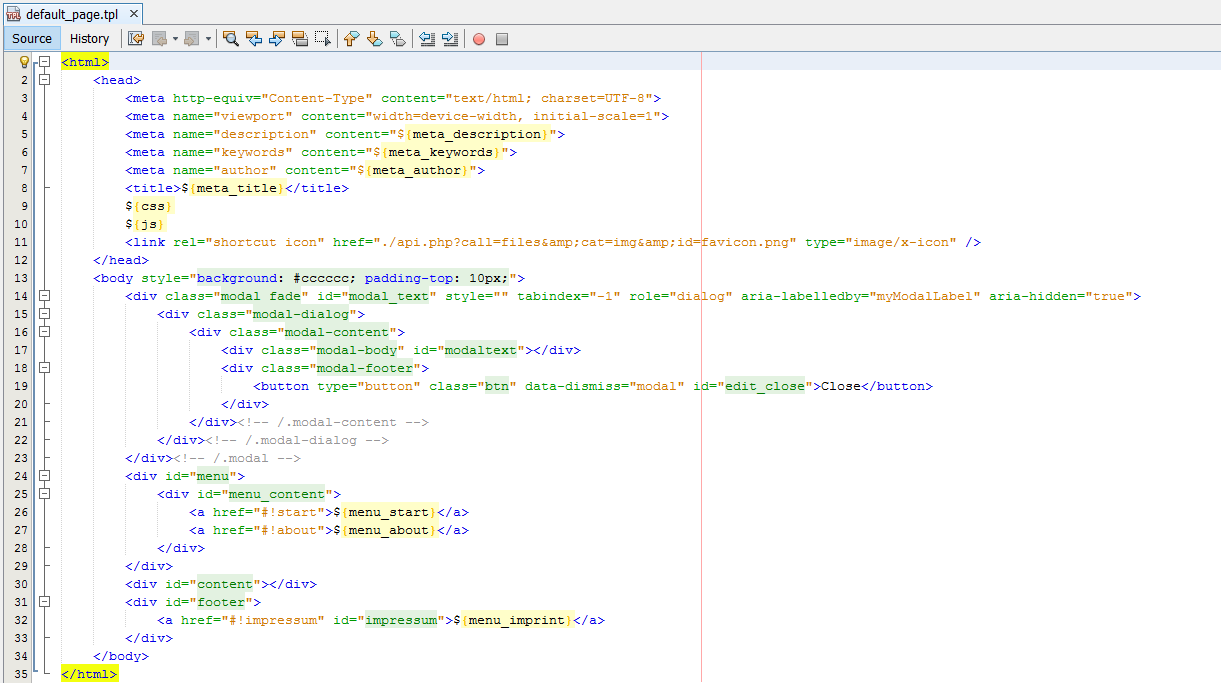
\includegraphics[width=10cm]{img/default_page_tpl.png}
	\end{backgroundblock}
}

\subsubsection*{Modulare GUI für administrative Aufgaben}
\frame{
	\frametitle{System Admin Interface - SAI}
	Das System Admin Interface verwaltet System Tabellen und Funktionalität.
	\begin{block}{}
	\begin{itemize}
	\item{Modular - erweiterbar}
	\item{Log - Alle fangbaren Fehler, die auf der Website auftreten}
	\item{Analysis - Besucher, Logins, Fehler}
	\item{Nutzerverwaltung}
	\item{Text, Cache, Cron, Config, Todo, Git, ...}
  	\end{itemize}
	\end{block}
}
\frame[t]{
	\frametitle{SAI - Start}
	\begin{backgroundblock}{1cm}{2.5cm}
		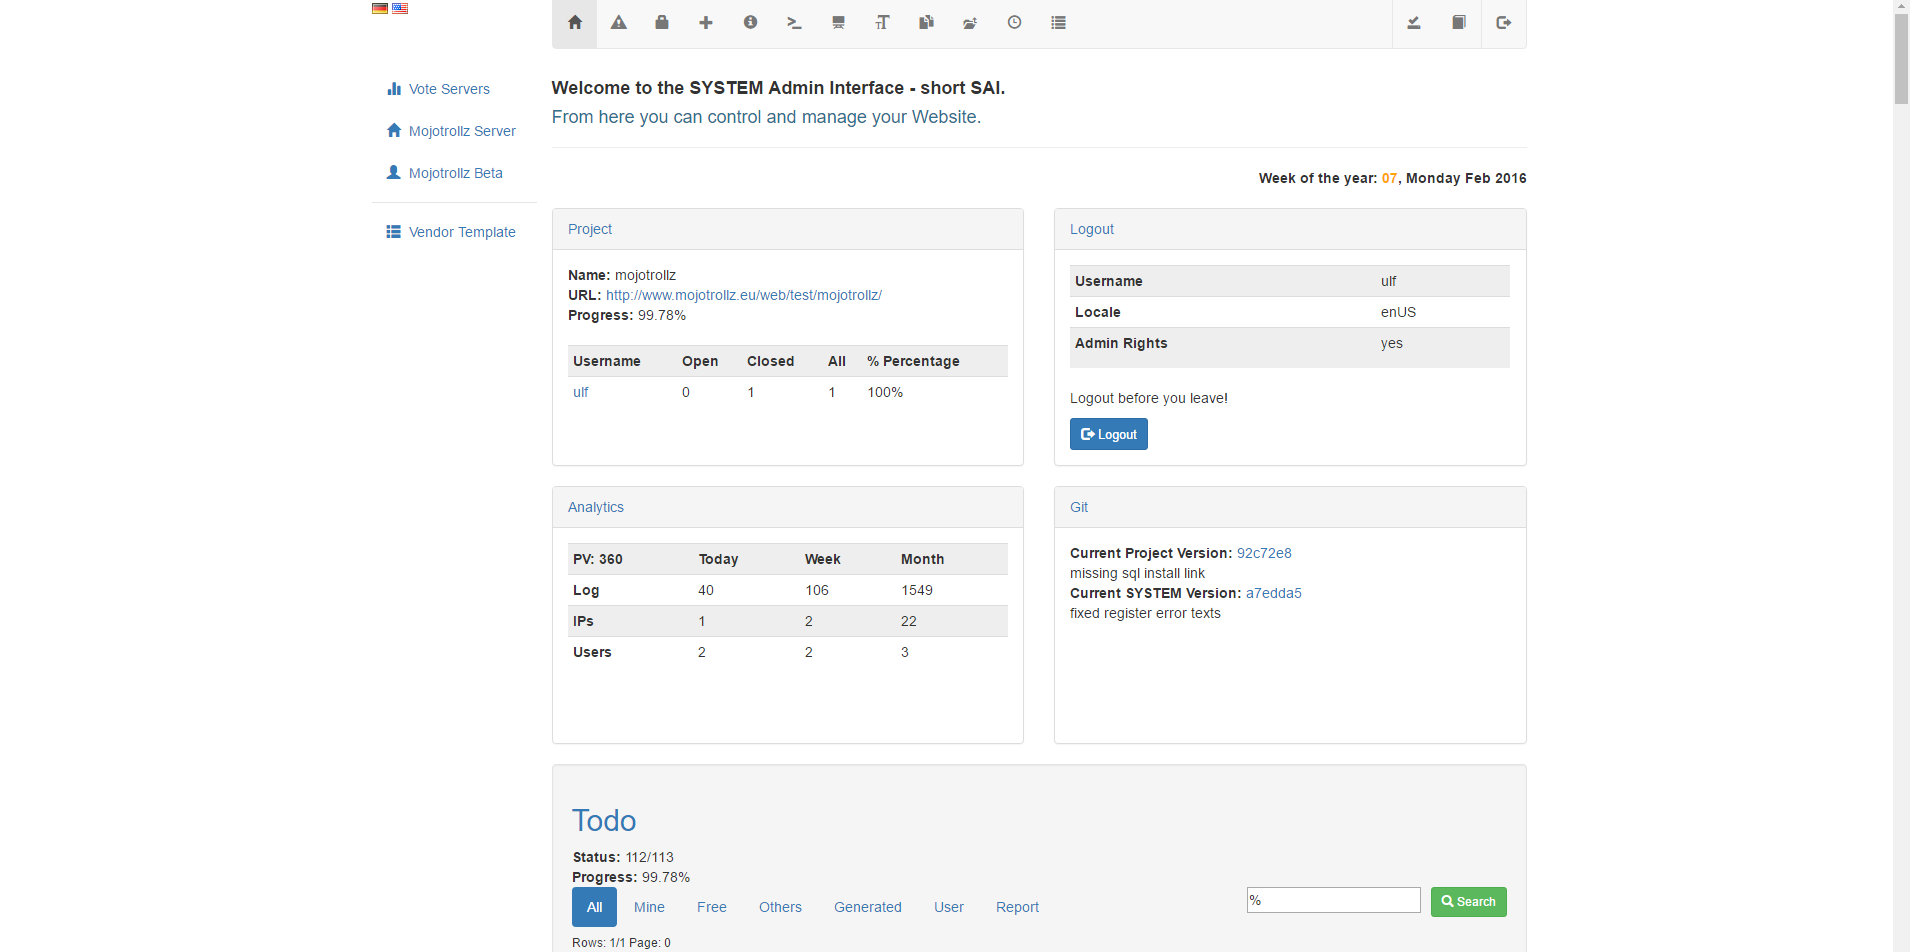
\includegraphics[width=10cm]{img/sai_start.png}
	\end{backgroundblock}
}
\frame[t]{
	\frametitle{SAI - Log}
	\begin{backgroundblock}{1cm}{2.5cm}
		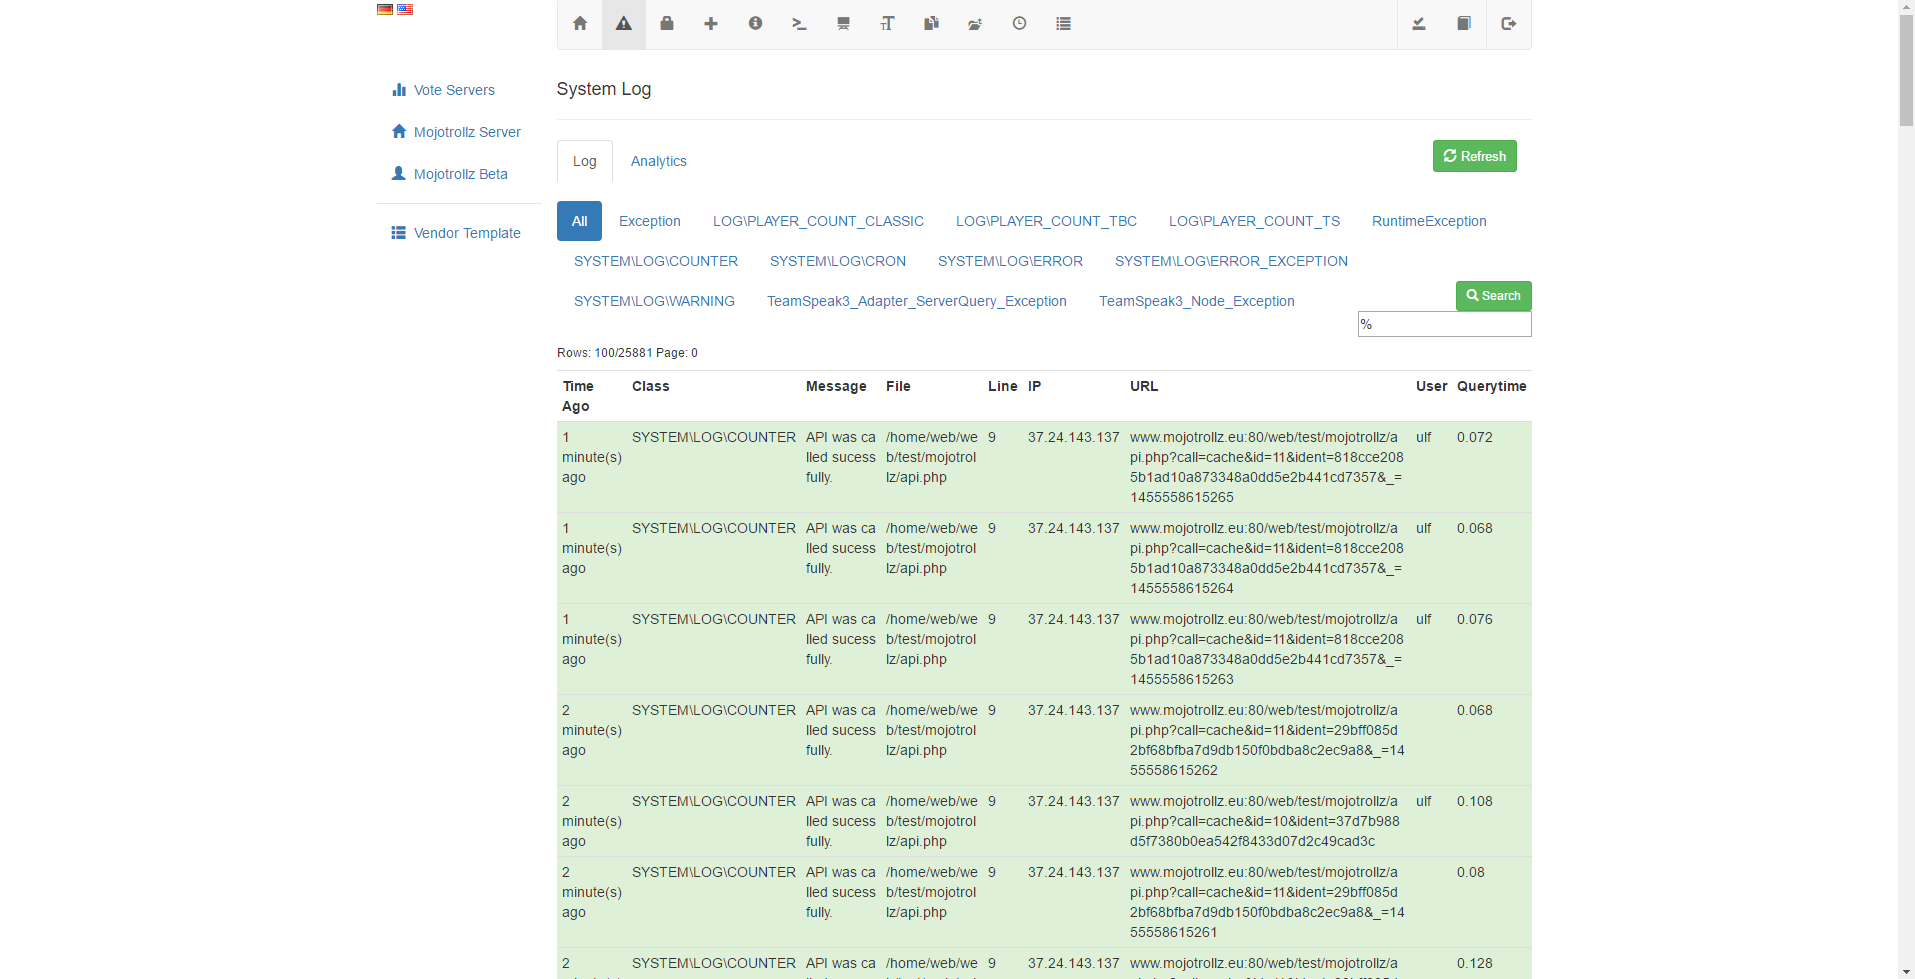
\includegraphics[width=10cm]{img/sai_log.png}
	\end{backgroundblock}
}
\frame[t]{
	\frametitle{SAI - Analysis}
	\begin{backgroundblock}{1cm}{2.5cm}
		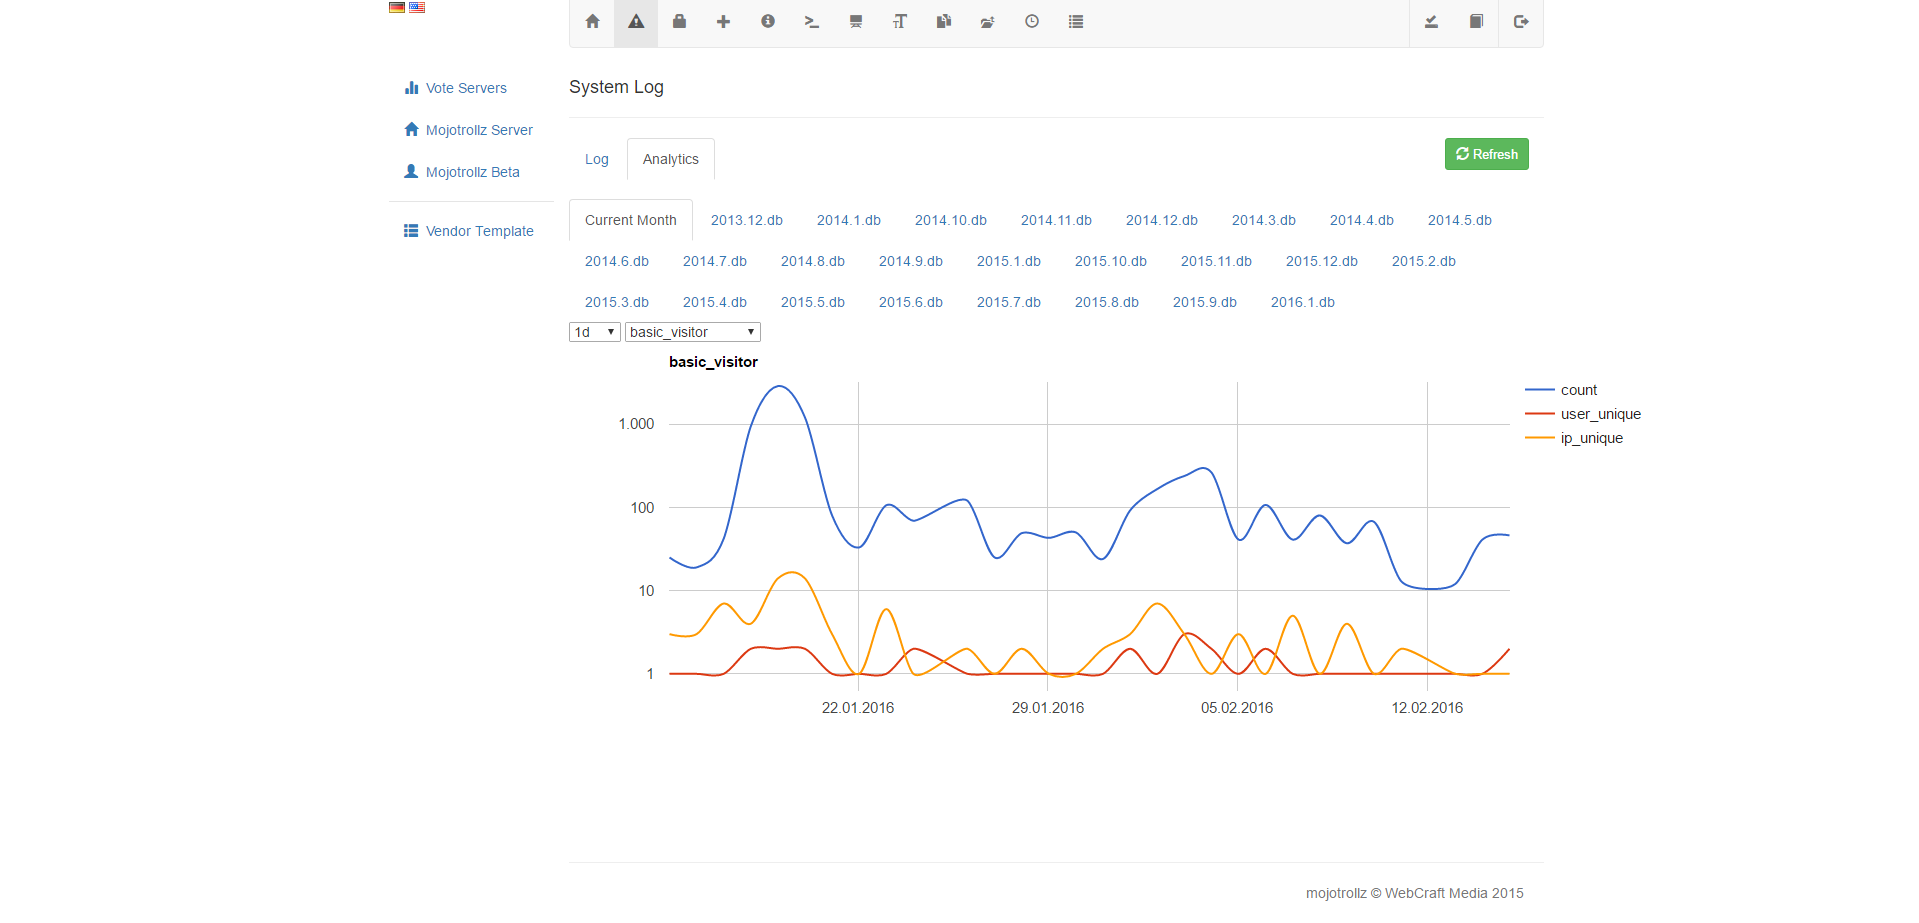
\includegraphics[width=10cm]{img/sai_analysis.png}
	\end{backgroundblock}
}
\frame[t]{
	\frametitle{SAI - Text}
	\begin{backgroundblock}{1cm}{2.5cm}
		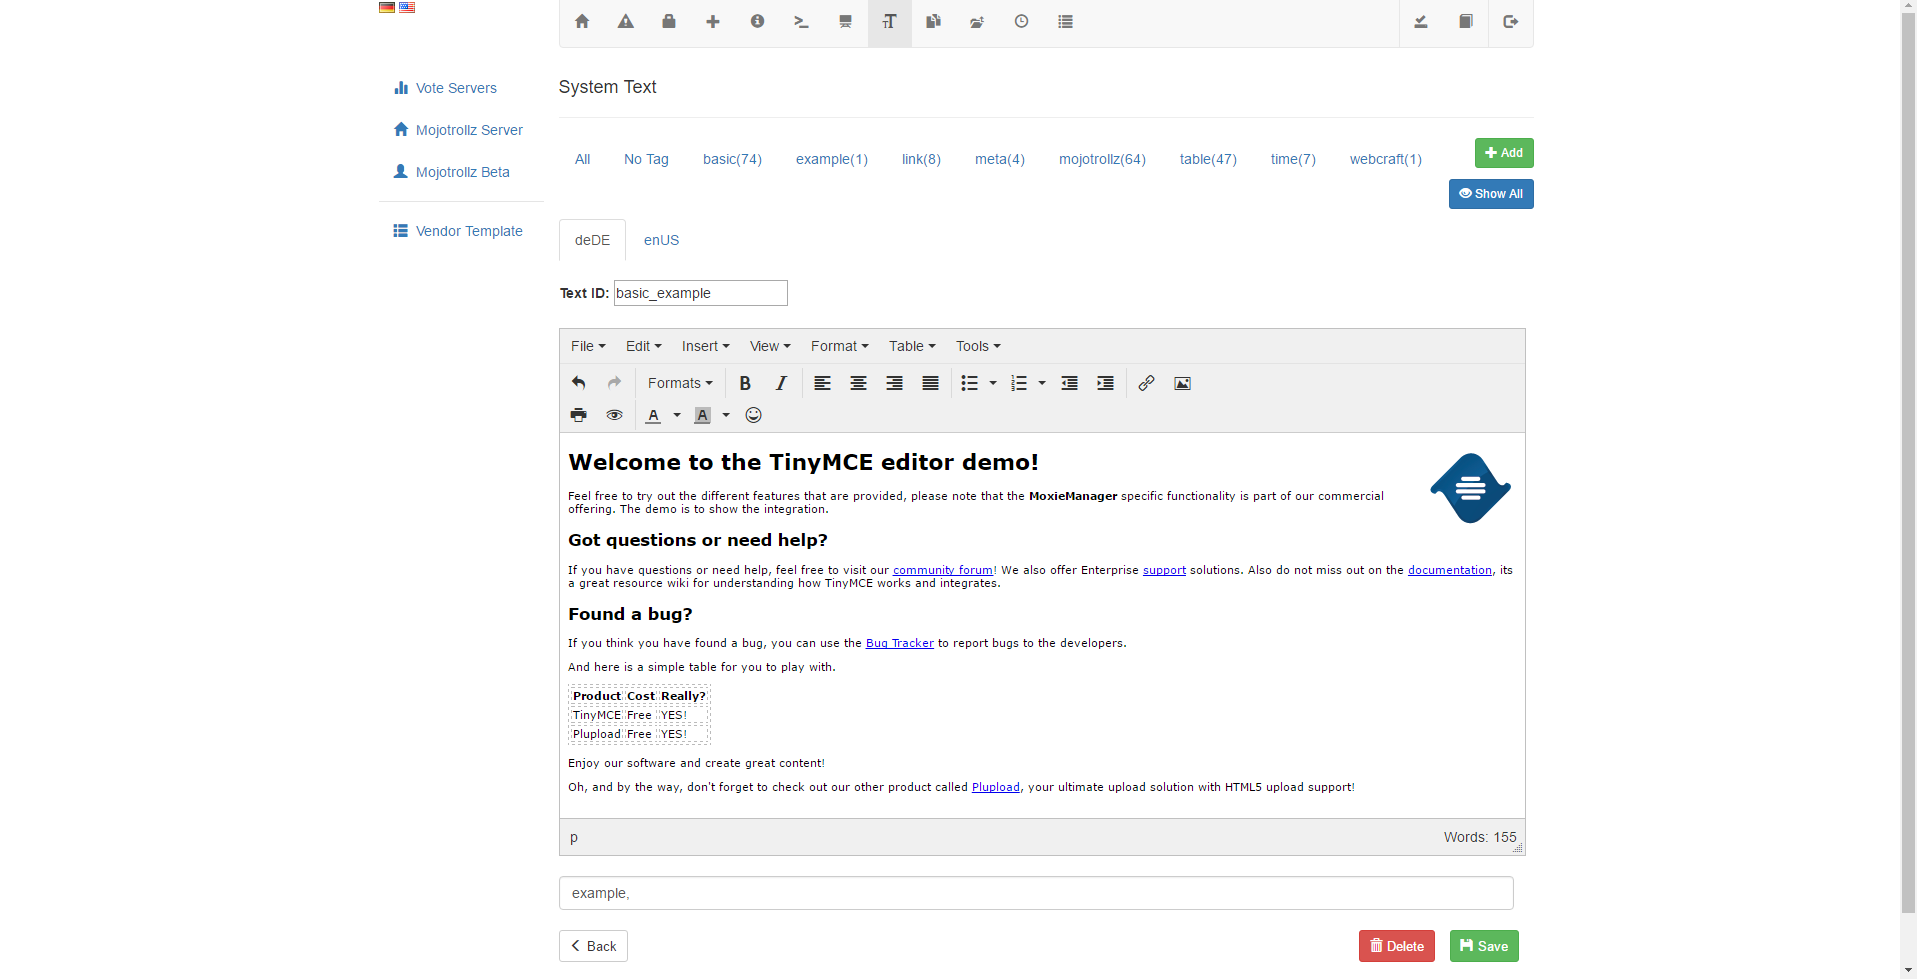
\includegraphics[width=10cm]{img/sai_text.png}
	\end{backgroundblock}
}
\frame[t]{
	\frametitle{SAI - Cron}
	\begin{backgroundblock}{1cm}{2.5cm}
		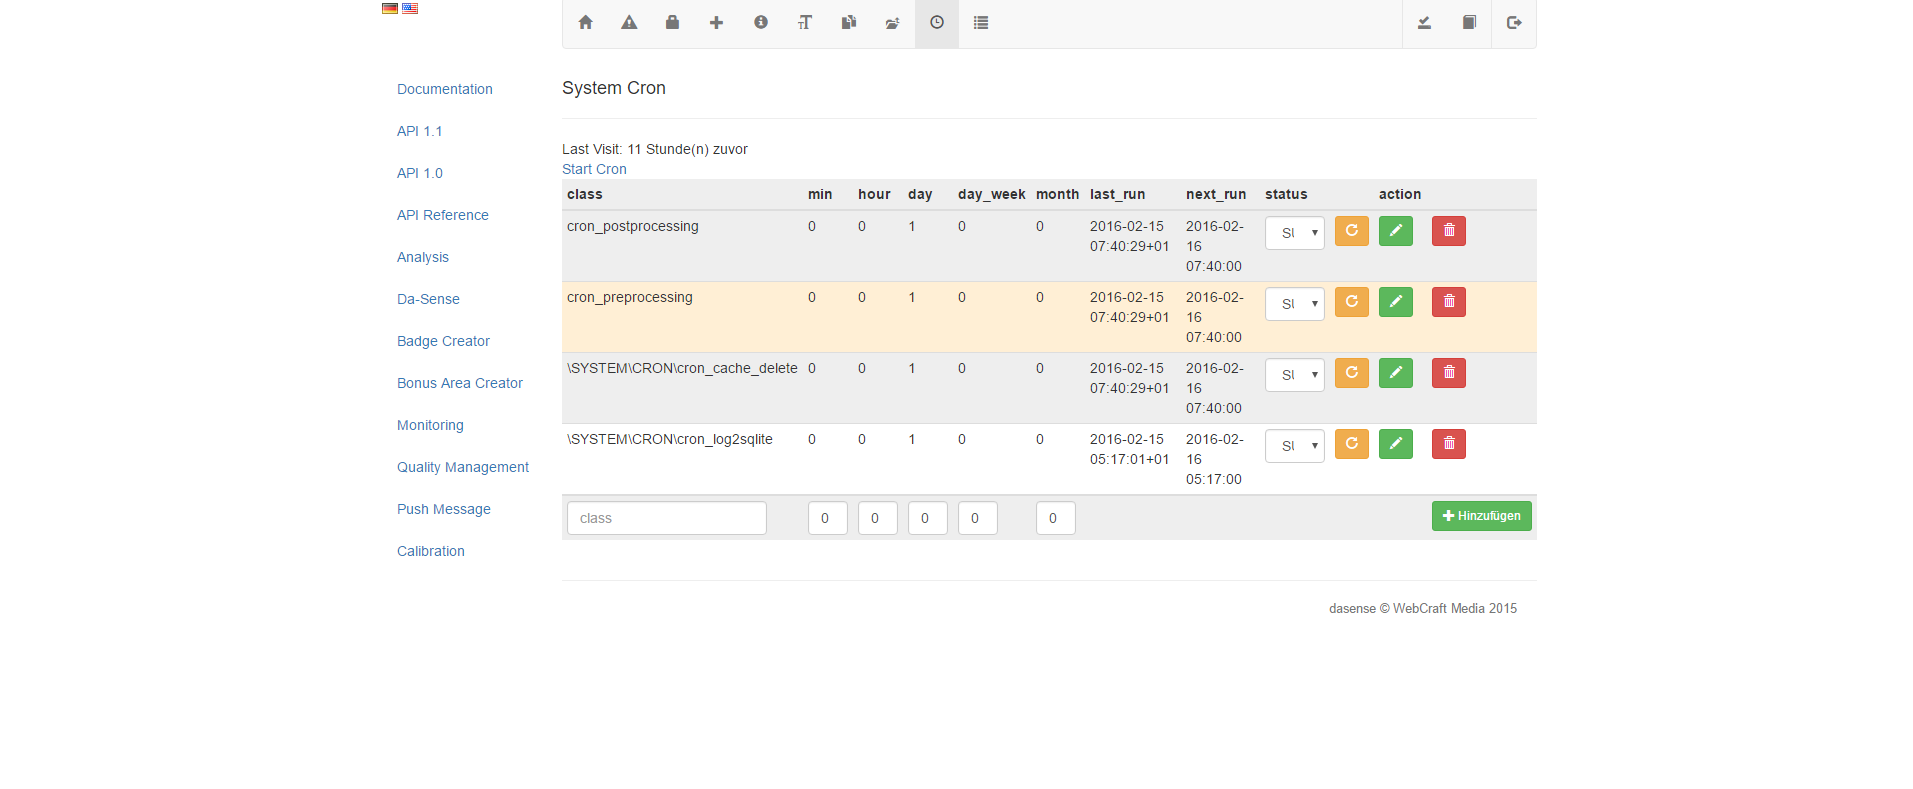
\includegraphics[width=10cm]{img/sai_cron.png}
	\end{backgroundblock}
}

\subsection{Vorteile und Nachteile}
\frame{					
	\begin{block}{Vorteile bei Einsatz von System}
	\begin{itemize}
	\item{Kompakt und Einfach}
	\item{Noch jung, keine starren Strukturen}
	\item{Git kompatibel}
	\item{frei (\url{https://github.com/webcraftmedia/system})}
  	\end{itemize}
	\end{block}
	\begin{block}{Nachteile bei Einsatz von System}
	\begin{itemize}
	\item{Geringe Verbreitung}
	\item{Geringer Anteil an Dokumentation}
	\item{Unzureichende Nutzerverwaltung}
  	\end{itemize}
	\end{block}
}

\subsection{Ausblick}
\frame[t]{
	\frametitle{Ausblick - Bootstrap}
	\begin{block}{}
	\begin{itemize}
	\item{Bootstrap Grid}
	\item{Col füllen/nachladen}
	\item{Bootstrap Menü}
  	\end{itemize}
	\end{block}
	\begin{block}{Nutzen}
	\begin{itemize}
	\item{``Click Click'' Websiten}
	\item{Noch einfacher}
	\item{Wiederverwertung von \\ Templates/Code}
  	\end{itemize}
	\end{block}
	\begin{backgroundblock}{6cm}{2.5cm}
		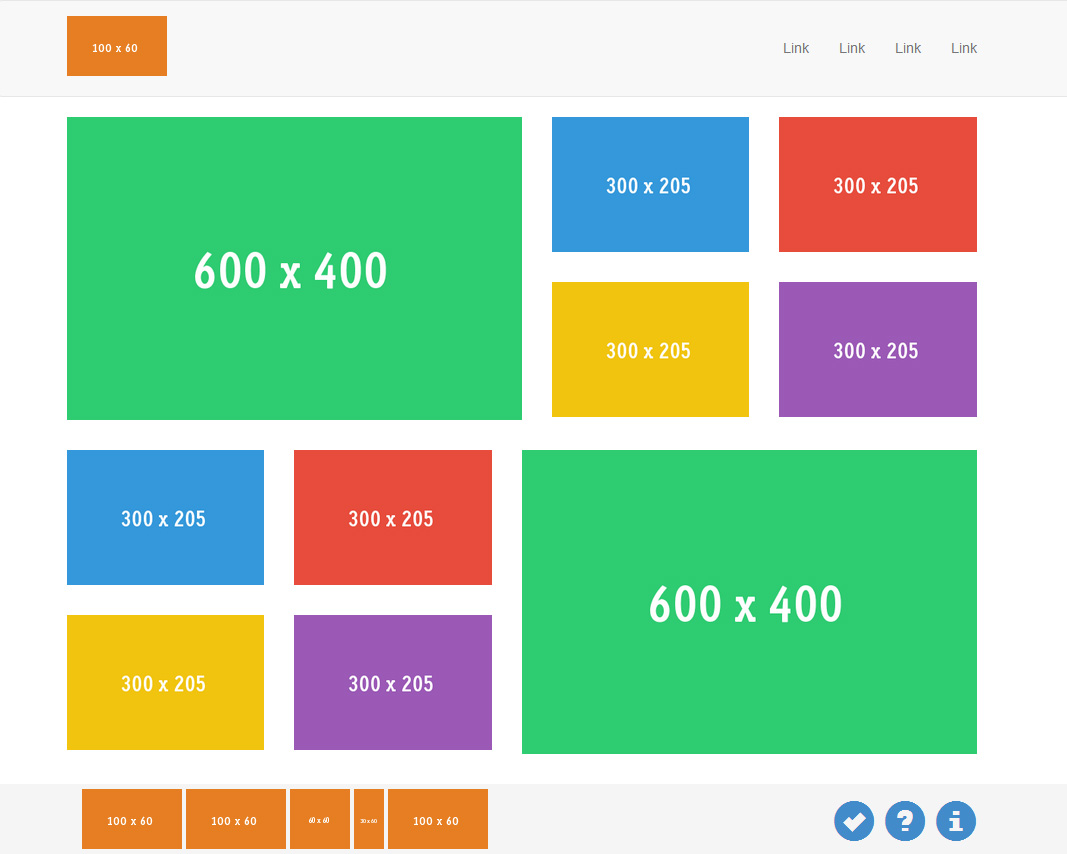
\includegraphics[width=6cm]{img/bootstrap_grid.jpg}
	\end{backgroundblock}
}
\frame{
	\frametitle{Ausblick - Usermanagement}
	\begin{block}{}
	\begin{itemize}
	\item{unzureichend}
	\item{umständlich}
	\item{Tabelle pro Projekt}
  	\end{itemize}
	\end{block}
	\begin{block}{SAML}
	\begin{itemize}
	\item{IDPs}
	\item{SPs}
	\item{verwaltung mehrer \\ Seiten, Zentralisierung}
  	\end{itemize}
	\end{block}
	\begin{backgroundblock}{6cm}{2.5cm}
		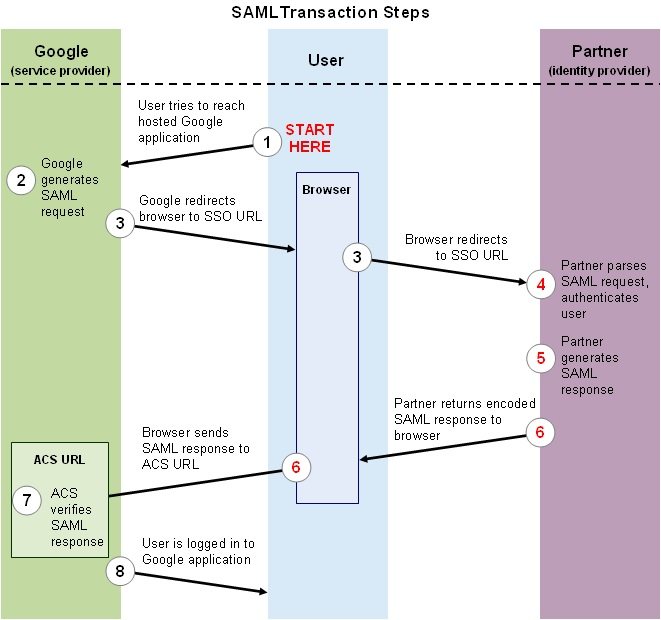
\includegraphics[width=6cm]{img/saml.jpg}
	\end{backgroundblock}
}